\documentclass[10pt]{article}\usepackage[]{graphicx}\usepackage[]{color}
%% maxwidth is the original width if it is less than linewidth
%% otherwise use linewidth (to make sure the graphics do not exceed the margin)
\makeatletter
\def\maxwidth{ %
  \ifdim\Gin@nat@width>\linewidth
    \linewidth
  \else
    \Gin@nat@width
  \fi
}
\makeatother

\definecolor{fgcolor}{rgb}{0.345, 0.345, 0.345}
\newcommand{\hlnum}[1]{\textcolor[rgb]{0.686,0.059,0.569}{#1}}%
\newcommand{\hlstr}[1]{\textcolor[rgb]{0.192,0.494,0.8}{#1}}%
\newcommand{\hlcom}[1]{\textcolor[rgb]{0.678,0.584,0.686}{\textit{#1}}}%
\newcommand{\hlopt}[1]{\textcolor[rgb]{0,0,0}{#1}}%
\newcommand{\hlstd}[1]{\textcolor[rgb]{0.345,0.345,0.345}{#1}}%
\newcommand{\hlkwa}[1]{\textcolor[rgb]{0.161,0.373,0.58}{\textbf{#1}}}%
\newcommand{\hlkwb}[1]{\textcolor[rgb]{0.69,0.353,0.396}{#1}}%
\newcommand{\hlkwc}[1]{\textcolor[rgb]{0.333,0.667,0.333}{#1}}%
\newcommand{\hlkwd}[1]{\textcolor[rgb]{0.737,0.353,0.396}{\textbf{#1}}}%
\let\hlipl\hlkwb

\usepackage{framed}
\makeatletter
\newenvironment{kframe}{%
 \def\at@end@of@kframe{}%
 \ifinner\ifhmode%
  \def\at@end@of@kframe{\end{minipage}}%
  \begin{minipage}{\columnwidth}%
 \fi\fi%
 \def\FrameCommand##1{\hskip\@totalleftmargin \hskip-\fboxsep
 \colorbox{shadecolor}{##1}\hskip-\fboxsep
     % There is no \\@totalrightmargin, so:
     \hskip-\linewidth \hskip-\@totalleftmargin \hskip\columnwidth}%
 \MakeFramed {\advance\hsize-\width
   \@totalleftmargin\z@ \linewidth\hsize
   \@setminipage}}%
 {\par\unskip\endMakeFramed%
 \at@end@of@kframe}
\makeatother

\definecolor{shadecolor}{rgb}{.97, .97, .97}
\definecolor{messagecolor}{rgb}{0, 0, 0}
\definecolor{warningcolor}{rgb}{1, 0, 1}
\definecolor{errorcolor}{rgb}{1, 0, 0}
\newenvironment{knitrout}{}{} % an empty environment to be redefined in TeX

\usepackage{alltt}
\usepackage[breaklinks=true]{hyperref}
\usepackage{url}
\usepackage[a4paper, margin = 1.5cm]{geometry}
\usepackage{a4wide}
\usepackage{float}
\usepackage[english]{babel}
\usepackage[utf8]{inputenc}
\usepackage{amsmath}
\usepackage{amssymb}
\usepackage[backend=bibtex,style=numeric-comp,sorting=none]{biblatex}
\bibliography{report}
\usepackage{subcaption}
\usepackage[font={small}]{caption}
\usepackage{booktabs}
\usepackage{listings}
\usepackage{cleveref}
\newcommand{\approxtext}[1]{\ensuremath{\stackrel{\text{#1}}{=}}}
\newcommand{\matr}[1]{\mathbf{#1}}
\newcommand{\partt}[2]{\ensuremath{\dfrac{\partial {#1}}{\partial {#2}}}}
\renewcommand{\d}[1]{\ensuremath{\operatorname{d}\!{#1}}} % non-italized differentials
\newcommand{\h}[0]{\ensuremath{\hbar}} % hbar
\def\changemargin#1#2{\list{}{\rightmargin#2\leftmargin#1}\item[]}
\let\endchangemargin=\endlist 
\usepackage{amsthm}
\theoremstyle{plain}
\renewcommand{\theequation}{\thesection.\arabic{equation}}
\def\changemargin#1#2{\list{}{\rightmargin#2\leftmargin#1}\item[]}
\let\endchangemargin=\endlist    
\newcommand{\ts}{\textsuperscript} 
% Stephen's stuff
\newcommand{\R}{\texttt{R}}
\newcommand{\Rfunction}[1]{{\texttt{#1}}}
\newcommand{\Robject}[1]{{\texttt{#1}}}
\newcommand{\Rpackage}[1]{{\mbox{\normalfont\textsf{#1}}}}
\usepackage{xcolor}
\definecolor{Red}{rgb}{0.7,0,0}
\definecolor{Blue}{rgb}{0,0,0.8}
\hypersetup{%
  pdfusetitle,
  bookmarks = {true},
  bookmarksnumbered = {true},
  bookmarksopen = {true},
  bookmarksopenlevel = 2,
  unicode = {true},
  breaklinks = {false},
  hyperindex = {true},
  colorlinks = {true},
  linktocpage = {true},
  plainpages = {false},
  linkcolor = {Blue},
  citecolor = {Blue},
  urlcolor = {Red},
  pdfstartview = {Fit},
  pdfpagemode = {UseOutlines},
  pdfview = {XYZ null null null}
}
%% Listings
\lstset{ 
  language=R,                     % the language of the code
  basicstyle=\footnotesize,       % the size of the fonts that are used for the code
  numbers=left,                   % where to put the line-numbers
  numberstyle=\tiny\color{gray},  % the style that is used for the line-numbers
  stepnumber=1,                   % the step between two line-numbers. If it's 1, each line will be numbered
  numbersep=5pt,                  % how far the line-numbers are from the code
  backgroundcolor=\color{white},  % choose the background color. You must add \usepackage{color}
  showspaces=false,               % show spaces adding particular underscores
  showstringspaces=false,         % underline spaces within strings
  showtabs=false,                 % show tabs within strings adding particular underscores
  rulecolor=\color{black},        % if not set, the frame-color may be changed on line-breaks within not-black text (e.g. commens (green here))
  tabsize=2,                      % sets default tabsize to 2 spaces
  captionpos=b,                   % sets the caption-position to bottom
  breaklines=true,                % sets automatic line breaking
  breakatwhitespace=false,        % sets if automatic breaks should only happen at whitespace
  title=\lstname,                 % show the filename of files included with \lstinputlisting;
                                  % also try caption instead of title
  keywordstyle=\color{blue},      % keyword style
  commentstyle=\color{green},   % comment style
  stringstyle=\color{purple},      % string literal style
  escapeinside={\%*}{*)},         % if you want to add a comment within your code
  morekeywords={*,...}            % if you want to add more keywords to the set
} 
\usepackage{verbatim}
\usepackage{multicol}
\def\changemargin#1#2{\list{}{\rightmargin#2\leftmargin#1}\item[]}
\let\endchangemargin=\endlist

%%%%%%%%%%%%%%%%%%%% Begin
\title
{
  %\phantom{a}\vspace{2cm}
	\textbf
	{
      Scientific Programming: Assignment 2
  }\\[1em]
  \small{University of Cambridge}
}

\author{Henrik Åhl}
\date{\today}
\IfFileExists{upquote.sty}{\usepackage{upquote}}{}
\begin{document}

\date{\today}
\maketitle
\setcounter{page}{1}
\begin{abstract}
\begin{changemargin}{-.8cm}{-.8cm}
{\bf
  We investigate weather data for Cambridge, Cambridgeshire, UK, gathered from the \textit{Digital Technology Group} at the University of Cambridge. The data spans from \date{1995-07-01} to \date{2016-10-25}, but contains multiple accuracies which are accounted for.
  
\hspace{.5cm}By filtering out missing data in the metrics of hours of sunshine, total amount of rain and temperature, we achieve a data set on which we perform various analyses, such as identification of the days which showed the higest respectively lowest average temperatures. 
}

\end{changemargin} 
\end{abstract}
%\begin{multicols*}{2}
\section*{Preface}
This is an assignment report in connection to the \textit{Scientific Programming} module in the Computational Biology course at the University of Cambridge, Michaelmas term 2016. All related code is as of \date{\today} available per request by contacting \href{mailto:hpa22@cam.ac.uk}{hpa22@cam.ac.uk}. Data used is hosted at \url{https://www.cl.cam.ac.uk/research/dtg/weather/index-daily-text.html}, and is freely accessible.

\section{Handling of Inaccuracies}
The data points which contained inaccuracies were accounted for in most of the cases, although ambiguity in the inaccuracy descriptions prevented from systematically handling this. In particular, the inaccuracy information mentions a breakdown of the rain sensor in October 2011, but is then not mentioned again aside of a remark regarding a temporary replacement. In this case, all data after this event are disregarded, as no specific breaking point could be determined. 

In other cases, when the inaccuracy page mentions breakdown of a certain metric, the dates for this are disregarded. Note, however, that a breakdown in for example the rain data sensor is not accounted for in analyses of the other metrics, in order to improve the data set. Futhermore, inaccuracies when the data management team express uncertainty about the quality of the data are not accounted for unless the data points show clearly faulty behavior.

In the case where the treatment is very ambiguous, the following choices have been made with respect to the corresponding metrics:
\begin{enumerate}
  \item A few data points have been corrected after initial insertion, rendering duplicate files (with copies having a '\textbackslash$\sim$' suffix). Only the corrected files are kept.
  \item We disregard the mentioned clock synchronisation error. All times are rounded to the nearest half-hour. Because of this, multiple data points for the same timestamp arise in some cases. We here choose to only keep the latest entered data point.
  \item The data management team voice concern about precipitation \date{2001-06-01} to \date{2001-07-29}, where it is mentioned that lower-value data points hold higher accuracy. We remove all data points in this interval.
  \item For dates \date{2006-10-05} to \date{2006-10-09}, we keep the data point for the 6th as it appears to have been manually corrected by the data management, but rid ourselves of the rest.
  \item Dates which are stated to have already been corrected are not removed from the analysis.
  \item A remark about possible inaccuracies due to a sun shield are mentioned, though as this is not something which is voiced as any greater concern, the data points corresponding to these dates are kept.
  \item All data was pruned with respect to faulty values. For example, some files contained placeholder asterisks. These timestamps were removed, and the data treated in accordance to previously stated methods.
\end{enumerate}

Finally, we must also note that our approach carries a few biases. In particular, in the case of a time-shift from summer to winter and \textit{vice versa}, our method of only keeping latter duplicates and complete datasets with respect to the number of time stamps will skew our analysis in that we will remove a complete day in half of the cases, and lose singular data points in the other half.

\section{Problems and Solutions}
\subsection{Filtering and file sizes}
The data were initially filtered using a 1000 bit file size limit, in order to to a further extent only account for directly relevant files. The files filtered for the analyses of \texttt{rain}, \texttt{sunshine} and \texttt{temperature} data can collectively be found in the appendix, along with statistics for the files used. 

\texttt{Rain} data was filtered mainly by the inaccuracies information page, and turned out to be the variable most frequently having technical issues. \texttt{Sunlight} was filtered by removing all data points with $> 16$ hours of sunlight recorded in a single day. We corrected \texttt{temperature} by removing all data points with temperatures $< -25$ or $> 35$. The temperature data set also shows a group of data points occuring in the late December to early January region, all having a mean temperatures of 11.4 $^\circ$C. However, as these could not be related to any noted malfunctions, and proved difficult to remove systematically, no corrections were made. Nevertheless, this does has an effect on the data, and can be seen causing spikes in particular in \cref{fig:compareYears} (see Dec--Feb).


\subsection{Temperature Data for Christmas Eve 2012}
\begin{knitrout}
\definecolor{shadecolor}{rgb}{0.969, 0.969, 0.969}\color{fgcolor}\begin{figure}[H]

{\centering 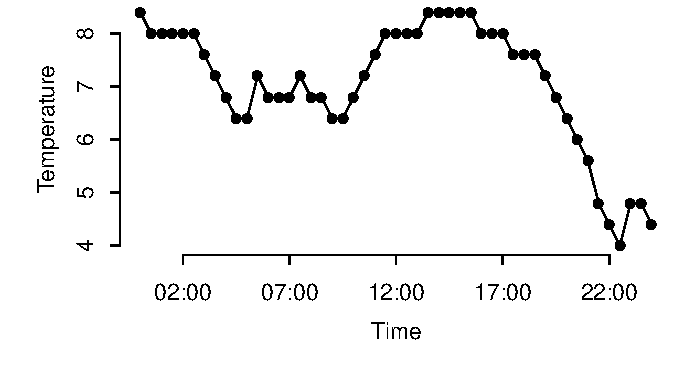
\includegraphics[width=\maxwidth]{figure/graphics-christmas-1} 

}

\caption[Temperature over 24 hours for Christmas Eve 2012]{Temperature over 24 hours for Christmas Eve 2012}\label{fig:christmas}
\end{figure}


\end{knitrout}
The temperature for Christmas Eve 2012 can be seen to start off at a surprisingly high temperature, subsequently falling off until it again starts increasing before noon. Shortly after mid-day, the temperature reaches its peak, whereafter it then falls towards even lower temperatures. 

\subsection{Mean Temperature as a Function of the Date}
\begin{knitrout}
\definecolor{shadecolor}{rgb}{0.969, 0.969, 0.969}\color{fgcolor}\begin{figure}[H]

{\centering 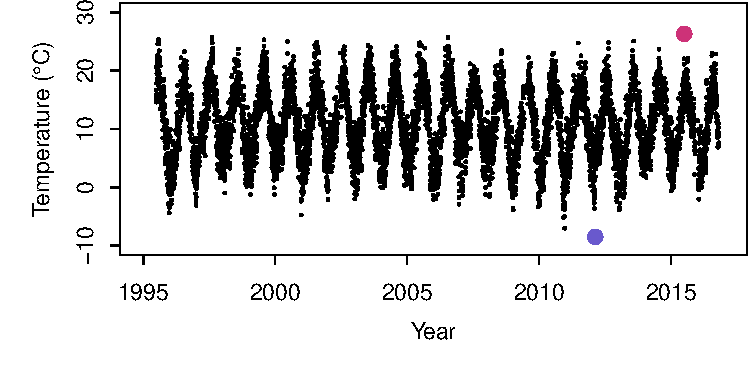
\includegraphics[width=\maxwidth]{figure/graphics-meantemp-1} 

}

\caption[Mean temperature for all (pruned) dates]{Mean temperature for all (pruned) dates. The enlarged dots signify the highest respectively lowest recorded mean temperature.}\label{fig:meantemp}
\end{figure}


\end{knitrout}

\Cref{fig:meantemp} shows the daily mean temperature for the data set. As expected, we see the oscillatory, stable behaviour of the temperature, ensuring that summer indeed returns to summer. The coldest respectively warmest day on average was found to be 2012-02-11 and 2015-07-01, who both can be seen as the enlarged, coloured dots in the graph.

\subsection{Mean of the mean temperatures}
\begin{knitrout}
\definecolor{shadecolor}{rgb}{0.969, 0.969, 0.969}\color{fgcolor}\begin{figure}[H]

{\centering 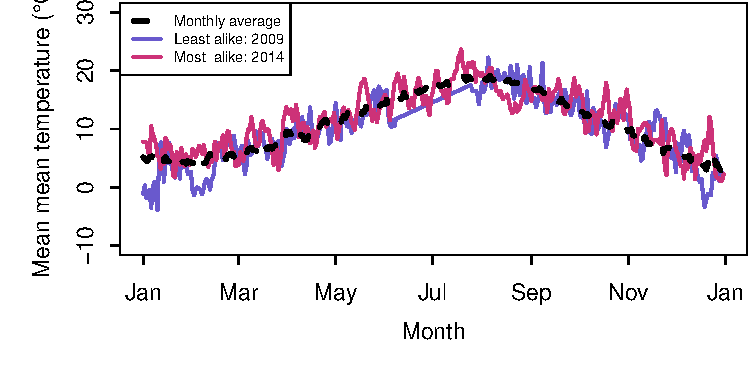
\includegraphics[width=\maxwidth]{figure/graphics-compareYears-1} 

}

\caption[Comparison between the average temperature for all (366) days in the calendar year]{Comparison between the average temperature for all (366) days in the calendar year. In red is shown the year most similar to the average, as measured by the summed squared distance for available data points. Conversely, the blue curve shows the least similar year.}\label{fig:compareYears}
\end{figure}


\end{knitrout}
The dotted line in \cref{fig:compareYears} shows the mean mean temperature for each individual day in the calendar year, given our data. Both the least on most similar annual temperature trajectory are seen as the two coloured lines, who as expected follow a more volatile path. These were determined using a summed squared distance method for all available data points. However, the years 1995 and 2016 were excluded due to only being partial.

The gap reaching from June to laste August in our year with the worst fit to the average is due to removal of data because of sensor malfunction. Note, however, that the points in this interval are not included in the summed distance measure. 

\subsection{Temperature--rain correlation}
\begin{knitrout}
\definecolor{shadecolor}{rgb}{0.969, 0.969, 0.969}\color{fgcolor}\begin{figure}[H]

{\centering 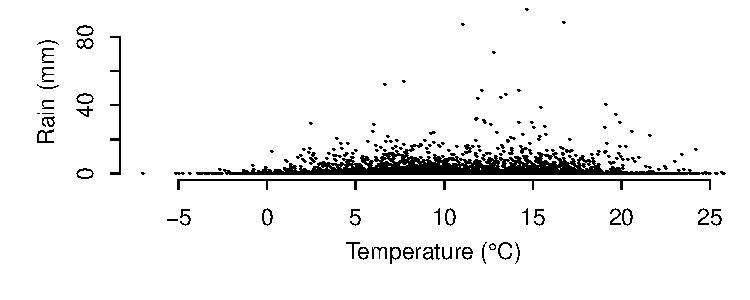
\includegraphics[width=\maxwidth]{figure/graphics-tempVSrain-1} 

}

\caption[Scatterplot for temperature-rain relationship]{Scatterplot for temperature-rain relationship.}\label{fig:tempVSrain}
\end{figure}


\end{knitrout}

As depicted in \cref{fig:tempVSrain} the relationship between temperature and rain show no significant features aside from an accumulation of data in the 2--20 $^\circ$C region. The Pearson correlation is 0.019.

\subsection{Temperature--sunlight relationship}
\begin{knitrout}
\definecolor{shadecolor}{rgb}{0.969, 0.969, 0.969}\color{fgcolor}\begin{figure}[H]

{\centering 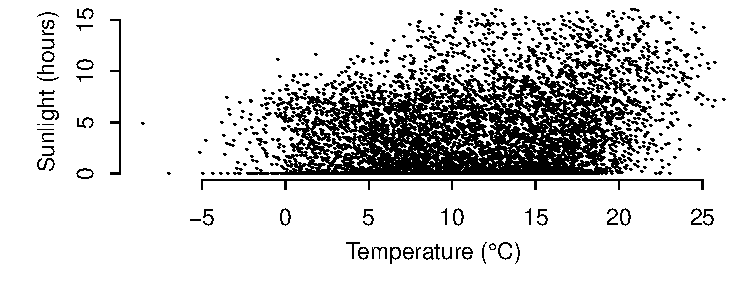
\includegraphics[width=\maxwidth]{figure/graphics-tempVSsun-1} 

}

\caption[Relationship between sunlight and mean daily temperature]{Relationship between sunlight and mean daily temperature.}\label{fig:tempVSsun}
\end{figure}


\end{knitrout}
In contrast to the rain--temperature data, temperature and sunlight are significantly more correlated. More specifically, the Pearson correlation is calculated to be 0.298.

\newpage
\subsection{Average min--max temperatures}
\begin{knitrout}
\definecolor{shadecolor}{rgb}{0.969, 0.969, 0.969}\color{fgcolor}\begin{figure}[H]

{\centering 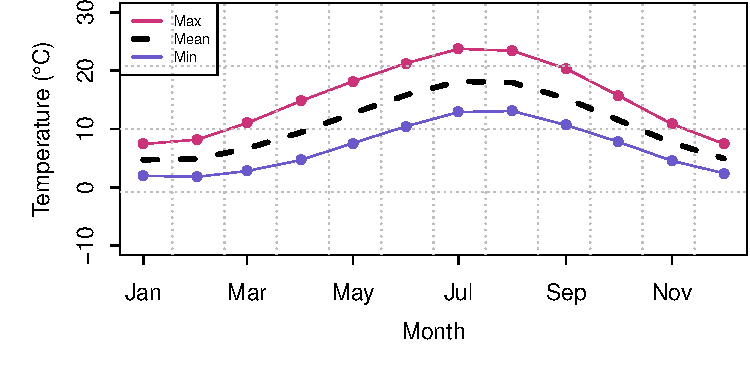
\includegraphics[width=\maxwidth]{figure/graphics-minMaxMonth-1} 

}

\caption[Monthly maximum, average and minimum values with respect to temperature]{Monthly maximum, average and minimum values with respect to temperature.}\label{fig:minMaxMonth}
\end{figure}


\end{knitrout}

Compared to the figure provided in the assignment notes, \cref{fig:minMaxMonth} displays high similarities. However, while July is the hottest month on average for both cases, the month with the lowest mean minimum is in our cases February. Also with respect to the absolute temperatures, our values are slightly upscaled. Most notably with respect to the high-summer months.

\subsection{A wet day}

We define a \textit{wet day} as one in which there falls at least 0.5~mm precipitation. Doing this, the highest number consequtive wet days are in the interval 1999-09-22 to 1999-09-30, i.e.\ making up an interval of length 9. We should nonetheless note that this result is highly affected by our treatment of the data, as intervals in which there are gaps are excluded. 

\printbibliography
%\end{multicols*}
\appendix
\section{Excluded dates}
\subsection{All data}

The total number of included files, i.e.\ the files with complete data in all categories, is ultimately 5397 files, which accounts for 70.2~\% of the initial file pool.

\subsection{Rain data}
The excluded \texttt{rain} data consists of 1955 files, making up 25.4~\% of the initial data set. The dates excluded are the following:
\begin{knitrout}
\definecolor{shadecolor}{rgb}{0.969, 0.969, 0.969}\color{fgcolor}\begin{kframe}
\begin{verbatim}
##    [1] "1998-04-14"  "2001-07-01"  "2001-07-02" 
##    [4] "2001-07-03"  "2001-07-04"  "2001-07-05" 
##    [7] "2001-07-06"  "2001-07-07"  "2001-07-08" 
##   [10] "2001-07-09"  "2001-07-10"  "2001-07-11" 
##   [13] "2001-07-12"  "2001-07-13"  "2001-07-14" 
##   [16] "2001-07-15"  "2001-07-16"  "2001-07-17" 
##   [19] "2001-07-18"  "2001-07-19"  "2001-07-20" 
##   [22] "2001-07-21"  "2001-07-22"  "2001-07-23" 
##   [25] "2001-07-24"  "2001-07-25"  "2001-07-26" 
##   [28] "2001-07-27"  "2001-07-28"  "2001-07-29" 
##   [31] "2001-07-30"  "2001-07-31"  "2001-08-01" 
##   [34] "2001-08-02"  "2001-08-03"  "2001-08-04" 
##   [37] "2001-08-05"  "2001-08-06"  "2001-08-07" 
##   [40] "2001-08-08"  "2001-08-09"  "2001-08-10" 
##   [43] "2001-08-11"  "2001-08-12"  "2001-08-13" 
##   [46] "2001-08-14"  "2001-08-15"  "2001-08-16" 
##   [49] "2001-08-17"  "2001-08-18"  "2001-08-19" 
##   [52] "2001-08-20"  "2001-08-21"  "2001-08-22" 
##   [55] "2001-08-23"  "2001-08-24"  "2001-08-25" 
##   [58] "2001-08-26"  "2001-08-27"  "2001-08-28" 
##   [61] "2001-08-29"  "2001-08-30"  "2001-08-31" 
##   [64] "2004-07-10"  "2004-07-11"  "2004-07-12" 
##   [67] "2004-07-13"  "2004-07-14"  "2004-07-15" 
##   [70] "2004-07-16"  "2004-07-17"  "2005-01-21" 
##   [73] "2005-01-22"  "2005-01-23"  "2005-01-24" 
##   [76] "2005-01-25"  "2005-01-26"  "2005-01-27" 
##   [79] "2005-01-28"  "2005-01-29"  "2005-01-30" 
##   [82] "2005-01-31"  "2005-02-01"  "2005-02-02" 
##   [85] "2005-02-03"  "2005-02-04"  "2005-02-05" 
##   [88] "2005-02-06"  "2005-02-07"  "2005-02-08" 
##   [91] "2005-02-09"  "2005-02-10"  "2005-02-11" 
##   [94] "2005-02-12"  "2005-02-13"  "2005-02-14" 
##   [97] "2005-02-15"  "2005-02-16"  "2005-02-17" 
##  [100] "2005-02-18"  "2005-02-19"  "2005-02-20" 
##  [103] "2005-02-21"  "2005-02-22"  "2005-02-23" 
##  [106] "2005-02-24"  "2005-02-25"  "2005-02-26" 
##  [109] "2005-02-27"  "2005-02-28"  "2005-03-01" 
##  [112] "2005-03-02"  "2005-06-30~" "2005-10-20" 
##  [115] "2005-10-21"  "2005-10-22"  "2005-10-23" 
##  [118] "2005-10-24"  "2005-10-26"  "2005-10-27" 
##  [121] "2005-10-28"  "2005-10-29"  "2005-10-30" 
##  [124] "2005-10-31"  "2005-11-01"  "2005-11-02" 
##  [127] "2005-11-03"  "2005-11-04"  "2005-11-05" 
##  [130] "2005-11-06"  "2005-11-07"  "2006-07-27" 
##  [133] "2006-07-28"  "2006-07-29"  "2006-07-30" 
##  [136] "2006-07-31"  "2006-10-07"  "2006-10-08" 
##  [139] "2006-10-09"  "2007-10-09"  "2007-10-10" 
##  [142] "2007-10-11"  "2007-10-12"  "2007-10-13" 
##  [145] "2007-10-14"  "2007-10-15"  "2007-10-16" 
##  [148] "2007-11-22"  "2008-08-03"  "2008-08-04" 
##  [151] "2008-08-12"  "2008-08-19"  "2008-08-20" 
##  [154] "2008-08-21"  "2008-08-23"  "2008-08-24" 
##  [157] "2008-08-25"  "2008-08-26"  "2008-08-27" 
##  [160] "2008-10-25"  "2008-10-27"  "2008-10-28" 
##  [163] "2008-10-30"  "2008-10-31"  "2008-11-01" 
##  [166] "2008-11-02"  "2008-11-03"  "2008-11-04" 
##  [169] "2009-04-10"  "2009-04-11"  "2009-04-12" 
##  [172] "2009-04-13"  "2010-02-06"  "2010-02-07" 
##  [175] "2010-02-08"  "2010-02-09"  "2010-02-10" 
##  [178] "2010-02-11"  "2010-02-12"  "2010-02-13" 
##  [181] "2010-02-14"  "2010-02-15"  "2010-02-16" 
##  [184] "2010-02-17"  "2010-02-18"  "2010-02-19" 
##  [187] "2010-02-20"  "2010-02-21"  "2010-02-22" 
##  [190] "2010-02-23"  "2010-02-24"  "2010-02-25" 
##  [193] "2010-02-26"  "2010-02-27"  "2010-02-28" 
##  [196] "2010-08-23"  "2011-02-26"  "2011-08-19" 
##  [199] "2011-08-20"  "2011-08-21"  "2011-08-22" 
##  [202] "2011-08-23"  "2011-09-06"  "2011-09-19" 
##  [205] "2011-09-20"  "2011-09-21"  "2011-09-22" 
##  [208] "2011-09-23"  "2011-09-24"  "2011-09-25" 
##  [211] "2011-09-26"  "2011-09-27"  "2011-09-28" 
##  [214] "2011-09-29"  "2011-09-30"  "2011-10-01" 
##  [217] "2011-10-02"  "2011-10-03"  "2011-10-04" 
##  [220] "2011-10-05"  "2011-10-06"  "2011-10-07" 
##  [223] "2011-10-08"  "2011-10-09"  "2011-10-10" 
##  [226] "2011-10-11"  "2011-10-12"  "2011-10-13" 
##  [229] "2011-10-14"  "2011-10-15"  "2011-10-16" 
##  [232] "2011-10-17"  "2011-10-18"  "2011-10-19" 
##  [235] "2011-10-20"  "2011-10-21"  "2011-10-22" 
##  [238] "2011-10-23"  "2011-10-24"  "2011-10-25" 
##  [241] "2011-10-26"  "2011-10-27"  "2011-10-28" 
##  [244] "2011-10-29"  "2011-11-01"  "2011-11-02" 
##  [247] "2011-11-03"  "2011-11-04"  "2011-11-05" 
##  [250] "2011-11-06"  "2011-11-07"  "2011-11-08" 
##  [253] "2011-11-09"  "2011-11-10"  "2011-11-11" 
##  [256] "2011-11-12"  "2011-11-13"  "2011-11-14" 
##  [259] "2011-11-15"  "2011-11-16"  "2011-11-17" 
##  [262] "2011-11-18"  "2011-11-19"  "2011-11-20" 
##  [265] "2011-11-21"  "2011-11-22"  "2011-11-23" 
##  [268] "2011-11-24"  "2011-11-26"  "2011-11-27" 
##  [271] "2011-11-28"  "2011-11-29"  "2011-11-30" 
##  [274] "2011-12-01"  "2011-12-02"  "2011-12-03" 
##  [277] "2011-12-04"  "2011-12-05"  "2011-12-07" 
##  [280] "2011-12-08"  "2011-12-09"  "2011-12-10" 
##  [283] "2011-12-11"  "2011-12-12"  "2011-12-13" 
##  [286] "2011-12-14"  "2011-12-15"  "2011-12-16" 
##  [289] "2011-12-17"  "2011-12-18"  "2011-12-19" 
##  [292] "2011-12-20"  "2011-12-21"  "2011-12-22" 
##  [295] "2011-12-23"  "2011-12-24"  "2011-12-25" 
##  [298] "2011-12-26"  "2011-12-27"  "2011-12-28" 
##  [301] "2011-12-29"  "2011-12-30"  "2011-12-31" 
##  [304] "2012-01-01"  "2012-01-02"  "2012-01-03" 
##  [307] "2012-01-04"  "2012-01-05"  "2012-01-06" 
##  [310] "2012-01-07"  "2012-01-08"  "2012-01-09" 
##  [313] "2012-01-11"  "2012-01-12"  "2012-01-13" 
##  [316] "2012-01-14"  "2012-01-15"  "2012-01-16" 
##  [319] "2012-01-17"  "2012-01-18"  "2012-01-19" 
##  [322] "2012-01-20"  "2012-01-21"  "2012-01-22" 
##  [325] "2012-01-23"  "2012-01-24"  "2012-01-25" 
##  [328] "2012-01-26"  "2012-01-27"  "2012-01-28" 
##  [331] "2012-01-29"  "2012-01-31"  "2012-02-01" 
##  [334] "2012-02-02"  "2012-02-03"  "2012-02-04" 
##  [337] "2012-02-05"  "2012-02-06"  "2012-02-07" 
##  [340] "2012-02-08"  "2012-02-09"  "2012-02-10" 
##  [343] "2012-02-11"  "2012-02-12"  "2012-02-13" 
##  [346] "2012-02-14"  "2012-02-15"  "2012-02-16" 
##  [349] "2012-02-17"  "2012-02-18"  "2012-02-19" 
##  [352] "2012-02-20"  "2012-02-21"  "2012-02-22" 
##  [355] "2012-02-23"  "2012-02-24"  "2012-02-25" 
##  [358] "2012-02-26"  "2012-02-27"  "2012-02-28" 
##  [361] "2012-02-29"  "2012-03-01"  "2012-03-02" 
##  [364] "2012-03-03"  "2012-03-04"  "2012-03-05" 
##  [367] "2012-03-06"  "2012-03-07"  "2012-03-08" 
##  [370] "2012-03-09"  "2012-03-10"  "2012-03-11" 
##  [373] "2012-03-12"  "2012-03-13"  "2012-03-14" 
##  [376] "2012-03-16"  "2012-03-17"  "2012-03-18" 
##  [379] "2012-03-19"  "2012-03-20"  "2012-03-21" 
##  [382] "2012-03-22"  "2012-03-23"  "2012-03-24" 
##  [385] "2012-03-26"  "2012-03-27"  "2012-03-28" 
##  [388] "2012-03-29"  "2012-03-30"  "2012-03-31" 
##  [391] "2012-04-01"  "2012-04-02"  "2012-04-03" 
##  [394] "2012-04-04"  "2012-04-05"  "2012-04-06" 
##  [397] "2012-04-07"  "2012-04-08"  "2012-04-09" 
##  [400] "2012-04-10"  "2012-04-11"  "2012-04-12" 
##  [403] "2012-04-13"  "2012-04-14"  "2012-04-15" 
##  [406] "2012-04-16"  "2012-04-17"  "2012-04-18" 
##  [409] "2012-04-21"  "2012-04-22"  "2012-04-23" 
##  [412] "2012-04-25"  "2012-04-26"  "2012-04-27" 
##  [415] "2012-04-28"  "2012-04-29"  "2012-04-30" 
##  [418] "2012-05-01"  "2012-05-02"  "2012-05-03" 
##  [421] "2012-05-04"  "2012-05-05"  "2012-05-06" 
##  [424] "2012-05-07"  "2012-05-08"  "2012-05-11" 
##  [427] "2012-05-12"  "2012-05-13"  "2012-05-14" 
##  [430] "2012-05-15"  "2012-05-16"  "2012-05-17" 
##  [433] "2012-05-18"  "2012-05-19"  "2012-05-20" 
##  [436] "2012-05-21"  "2012-05-22"  "2012-05-23" 
##  [439] "2012-05-24"  "2012-05-25"  "2012-05-26" 
##  [442] "2012-05-27"  "2012-05-28"  "2012-05-29" 
##  [445] "2012-05-30"  "2012-05-31"  "2012-06-01" 
##  [448] "2012-06-02"  "2012-06-03"  "2012-06-04" 
##  [451] "2012-06-05"  "2012-06-06"  "2012-06-07" 
##  [454] "2012-06-08"  "2012-06-09"  "2012-06-10" 
##  [457] "2012-06-11"  "2012-06-12"  "2012-06-13" 
##  [460] "2012-06-14"  "2012-06-15"  "2012-06-17" 
##  [463] "2012-06-18"  "2012-06-19"  "2012-06-20" 
##  [466] "2012-06-21"  "2012-06-22"  "2012-06-23" 
##  [469] "2012-06-24"  "2012-06-25"  "2012-06-26" 
##  [472] "2012-06-27"  "2012-06-28"  "2012-06-29" 
##  [475] "2012-06-30"  "2012-07-01"  "2012-07-02" 
##  [478] "2012-07-03"  "2012-07-04"  "2012-07-05" 
##  [481] "2012-07-06"  "2012-07-07"  "2012-07-08" 
##  [484] "2012-07-09"  "2012-07-10"  "2012-07-11" 
##  [487] "2012-07-12"  "2012-07-13"  "2012-07-14" 
##  [490] "2012-07-15"  "2012-07-16"  "2012-07-17" 
##  [493] "2012-07-18"  "2012-07-19"  "2012-07-20" 
##  [496] "2012-07-21"  "2012-07-22"  "2012-07-23" 
##  [499] "2012-07-24"  "2012-07-25"  "2012-07-26" 
##  [502] "2012-07-27"  "2012-07-28"  "2012-07-29" 
##  [505] "2012-07-30"  "2012-07-31"  "2012-08-01" 
##  [508] "2012-08-02"  "2012-08-03"  "2012-08-04" 
##  [511] "2012-08-05"  "2012-08-06"  "2012-08-07" 
##  [514] "2012-08-08"  "2012-08-09"  "2012-08-10" 
##  [517] "2012-08-11"  "2012-08-12"  "2012-08-13" 
##  [520] "2012-08-14"  "2012-08-15"  "2012-08-16" 
##  [523] "2012-08-17"  "2012-08-18"  "2012-08-19" 
##  [526] "2012-08-20"  "2012-08-21"  "2012-08-22" 
##  [529] "2012-08-23"  "2012-08-24"  "2012-08-25" 
##  [532] "2012-08-26"  "2012-08-27"  "2012-08-28" 
##  [535] "2012-08-29"  "2012-08-30"  "2012-08-31" 
##  [538] "2012-09-01"  "2012-09-02"  "2012-09-03" 
##  [541] "2012-09-04"  "2012-09-05"  "2012-09-06" 
##  [544] "2012-09-07"  "2012-09-08"  "2012-09-09" 
##  [547] "2012-09-10"  "2012-09-11"  "2012-09-12" 
##  [550] "2012-09-13"  "2012-09-14"  "2012-09-15" 
##  [553] "2012-09-16"  "2012-09-17"  "2012-09-18" 
##  [556] "2012-09-19"  "2012-09-20"  "2012-09-21" 
##  [559] "2012-09-22"  "2012-09-23"  "2012-09-24" 
##  [562] "2012-09-25"  "2012-09-26"  "2012-09-27" 
##  [565] "2012-09-28"  "2012-09-29"  "2012-09-30" 
##  [568] "2012-10-01"  "2012-10-02"  "2012-10-03" 
##  [571] "2012-10-04"  "2012-10-05"  "2012-10-06" 
##  [574] "2012-10-07"  "2012-10-08"  "2012-10-09" 
##  [577] "2012-10-10"  "2012-10-11"  "2012-10-12" 
##  [580] "2012-10-14"  "2012-10-15"  "2012-10-16" 
##  [583] "2012-10-17"  "2012-10-18"  "2012-10-19" 
##  [586] "2012-10-20"  "2012-10-21"  "2012-10-22" 
##  [589] "2012-10-23"  "2012-10-24"  "2012-10-25" 
##  [592] "2012-10-26"  "2012-10-27"  "2012-10-29" 
##  [595] "2012-10-30"  "2012-10-31"  "2012-11-01" 
##  [598] "2012-11-02"  "2012-11-05"  "2012-11-06" 
##  [601] "2012-11-07"  "2012-11-08"  "2012-11-09" 
##  [604] "2012-11-10"  "2012-11-11"  "2012-11-12" 
##  [607] "2012-11-13"  "2012-11-14"  "2012-11-15" 
##  [610] "2012-11-16"  "2012-11-17"  "2012-11-18" 
##  [613] "2012-11-19"  "2012-11-20"  "2012-11-21" 
##  [616] "2012-11-22"  "2012-11-23"  "2012-11-24" 
##  [619] "2012-11-25"  "2012-11-27"  "2012-11-28" 
##  [622] "2012-11-29"  "2012-11-30"  "2012-12-01" 
##  [625] "2012-12-02"  "2012-12-03"  "2012-12-04" 
##  [628] "2012-12-05"  "2012-12-06"  "2012-12-07" 
##  [631] "2012-12-08"  "2012-12-09"  "2012-12-10" 
##  [634] "2012-12-11"  "2012-12-12"  "2012-12-13" 
##  [637] "2012-12-14"  "2012-12-15"  "2012-12-16" 
##  [640] "2012-12-17"  "2012-12-18"  "2012-12-19" 
##  [643] "2012-12-20"  "2012-12-21"  "2012-12-22" 
##  [646] "2012-12-23"  "2012-12-24"  "2012-12-25" 
##  [649] "2012-12-26"  "2012-12-27"  "2012-12-28" 
##  [652] "2012-12-29"  "2012-12-30"  "2012-12-31" 
##  [655] "2013-01-01"  "2013-01-02"  "2013-01-03" 
##  [658] "2013-01-04"  "2013-01-05"  "2013-01-06" 
##  [661] "2013-01-07"  "2013-01-08"  "2013-01-09" 
##  [664] "2013-01-10"  "2013-01-11"  "2013-01-12" 
##  [667] "2013-01-13"  "2013-01-14"  "2013-01-15" 
##  [670] "2013-01-16"  "2013-01-17"  "2013-01-18" 
##  [673] "2013-01-19"  "2013-01-20"  "2013-01-21" 
##  [676] "2013-01-22"  "2013-01-23"  "2013-01-24" 
##  [679] "2013-01-25"  "2013-01-26"  "2013-01-27" 
##  [682] "2013-01-28"  "2013-01-29"  "2013-01-30" 
##  [685] "2013-01-31"  "2013-02-01"  "2013-02-02" 
##  [688] "2013-02-03"  "2013-02-04"  "2013-02-05" 
##  [691] "2013-02-06"  "2013-02-07"  "2013-02-08" 
##  [694] "2013-02-09"  "2013-02-10"  "2013-02-13" 
##  [697] "2013-02-14"  "2013-02-15"  "2013-02-16" 
##  [700] "2013-02-17"  "2013-02-18"  "2013-02-19" 
##  [703] "2013-02-20"  "2013-02-21"  "2013-02-22" 
##  [706] "2013-02-23"  "2013-02-24"  "2013-02-25" 
##  [709] "2013-02-26"  "2013-02-27"  "2013-02-28" 
##  [712] "2013-03-01"  "2013-03-02"  "2013-03-03" 
##  [715] "2013-03-04"  "2013-03-05"  "2013-03-06" 
##  [718] "2013-03-07"  "2013-03-08"  "2013-03-09" 
##  [721] "2013-03-10"  "2013-03-11"  "2013-03-13" 
##  [724] "2013-03-14"  "2013-03-15"  "2013-03-16" 
##  [727] "2013-03-17"  "2013-03-18"  "2013-03-19" 
##  [730] "2013-03-20"  "2013-03-21"  "2013-03-22" 
##  [733] "2013-03-23"  "2013-03-24"  "2013-03-25" 
##  [736] "2013-03-26"  "2013-03-27"  "2013-03-28" 
##  [739] "2013-03-29"  "2013-03-30"  "2013-04-01" 
##  [742] "2013-04-02"  "2013-04-03"  "2013-04-04" 
##  [745] "2013-04-05"  "2013-04-06"  "2013-04-07" 
##  [748] "2013-04-08"  "2013-04-09"  "2013-04-10" 
##  [751] "2013-04-11"  "2013-04-12"  "2013-04-13" 
##  [754] "2013-04-14"  "2013-04-15"  "2013-04-17" 
##  [757] "2013-04-18"  "2013-04-19"  "2013-04-20" 
##  [760] "2013-04-21"  "2013-04-22"  "2013-04-23" 
##  [763] "2013-04-24"  "2013-04-25"  "2013-04-26" 
##  [766] "2013-04-27"  "2013-04-28"  "2013-04-29" 
##  [769] "2013-04-30"  "2013-05-01"  "2013-05-02" 
##  [772] "2013-05-03"  "2013-05-04"  "2013-05-05" 
##  [775] "2013-05-06"  "2013-05-07"  "2013-05-08" 
##  [778] "2013-05-09"  "2013-05-10"  "2013-05-11" 
##  [781] "2013-05-12"  "2013-05-13"  "2013-05-14" 
##  [784] "2013-05-15"  "2013-05-16"  "2013-05-17" 
##  [787] "2013-05-18"  "2013-05-19"  "2013-05-20" 
##  [790] "2013-05-21"  "2013-05-22"  "2013-05-23" 
##  [793] "2013-05-24"  "2013-05-25"  "2013-05-26" 
##  [796] "2013-05-27"  "2013-05-28"  "2013-05-29" 
##  [799] "2013-05-30"  "2013-05-31"  "2013-06-01" 
##  [802] "2013-06-02"  "2013-06-03"  "2013-06-04" 
##  [805] "2013-06-05"  "2013-06-06"  "2013-06-07" 
##  [808] "2013-06-08"  "2013-06-09"  "2013-06-10" 
##  [811] "2013-06-11"  "2013-06-12"  "2013-06-13" 
##  [814] "2013-06-14"  "2013-06-15"  "2013-06-16" 
##  [817] "2013-06-17"  "2013-06-18"  "2013-06-19" 
##  [820] "2013-06-20"  "2013-06-22"  "2013-06-23" 
##  [823] "2013-06-24"  "2013-06-25"  "2013-06-26" 
##  [826] "2013-06-27"  "2013-06-28"  "2013-06-29" 
##  [829] "2013-06-30"  "2013-07-01"  "2013-07-02" 
##  [832] "2013-07-03"  "2013-07-04"  "2013-07-05" 
##  [835] "2013-07-06"  "2013-07-07"  "2013-07-09" 
##  [838] "2013-07-10"  "2013-07-11"  "2013-07-12" 
##  [841] "2013-07-13"  "2013-07-14"  "2013-07-15" 
##  [844] "2013-07-16"  "2013-07-17"  "2013-07-18" 
##  [847] "2013-07-19"  "2013-07-20"  "2013-07-21" 
##  [850] "2013-07-22"  "2013-07-23"  "2013-07-24" 
##  [853] "2013-07-25"  "2013-07-26"  "2013-07-27" 
##  [856] "2013-07-28"  "2013-07-29"  "2013-07-30" 
##  [859] "2013-07-31"  "2013-08-01"  "2013-08-02" 
##  [862] "2013-08-03"  "2013-08-04"  "2013-08-05" 
##  [865] "2013-08-06"  "2013-08-07"  "2013-08-08" 
##  [868] "2013-08-09"  "2013-08-10"  "2013-08-11" 
##  [871] "2013-08-12"  "2013-08-13"  "2013-08-14" 
##  [874] "2013-08-15"  "2013-08-16"  "2013-08-17" 
##  [877] "2013-08-18"  "2013-08-19"  "2013-08-20" 
##  [880] "2013-08-21"  "2013-08-22"  "2013-08-23" 
##  [883] "2013-08-24"  "2013-08-25"  "2013-08-26" 
##  [886] "2013-08-27"  "2013-08-28"  "2013-08-29" 
##  [889] "2013-08-30"  "2013-08-31"  "2013-09-01" 
##  [892] "2013-09-02"  "2013-09-03"  "2013-09-04" 
##  [895] "2013-09-05"  "2013-09-09"  "2013-09-11" 
##  [898] "2013-09-12"  "2013-09-13"  "2013-09-14" 
##  [901] "2013-09-15"  "2013-09-16"  "2013-09-17" 
##  [904] "2013-09-18"  "2013-09-21"  "2013-09-24" 
##  [907] "2013-09-28"  "2013-09-29"  "2013-09-30" 
##  [910] "2013-10-01"  "2013-10-02"  "2013-10-04" 
##  [913] "2013-10-05"  "2013-10-06"  "2013-10-07" 
##  [916] "2013-10-08"  "2013-10-09"  "2013-10-10" 
##  [919] "2013-10-11"  "2013-10-12"  "2013-10-13" 
##  [922] "2013-10-14"  "2013-10-15"  "2013-10-16" 
##  [925] "2013-10-17"  "2013-10-18"  "2013-10-19" 
##  [928] "2013-10-20"  "2013-10-21"  "2013-10-22" 
##  [931] "2013-10-23"  "2013-10-24"  "2013-10-25" 
##  [934] "2013-10-26"  "2013-10-28"  "2013-10-29" 
##  [937] "2013-10-30"  "2013-10-31"  "2013-11-01" 
##  [940] "2013-11-02"  "2013-11-03"  "2013-11-04" 
##  [943] "2013-11-05"  "2013-11-06"  "2013-11-07" 
##  [946] "2013-11-08"  "2013-11-09"  "2013-11-10" 
##  [949] "2013-11-11"  "2013-11-12"  "2013-11-13" 
##  [952] "2013-11-14"  "2013-11-15"  "2013-11-16" 
##  [955] "2013-11-17"  "2013-11-18"  "2013-11-19" 
##  [958] "2013-11-20"  "2013-11-21"  "2013-11-22" 
##  [961] "2013-11-23"  "2013-11-24"  "2013-11-25" 
##  [964] "2013-11-26"  "2013-11-27"  "2013-11-28" 
##  [967] "2013-11-29"  "2013-11-30"  "2013-12-01" 
##  [970] "2013-12-02"  "2013-12-03"  "2013-12-04" 
##  [973] "2013-12-05"  "2013-12-06"  "2013-12-07" 
##  [976] "2013-12-08"  "2013-12-09"  "2013-12-10" 
##  [979] "2013-12-11"  "2013-12-12"  "2013-12-13" 
##  [982] "2013-12-14"  "2013-12-15"  "2013-12-16" 
##  [985] "2013-12-17"  "2013-12-18"  "2013-12-19" 
##  [988] "2013-12-20"  "2013-12-21"  "2013-12-22" 
##  [991] "2013-12-23"  "2013-12-24"  "2013-12-25" 
##  [994] "2013-12-26"  "2013-12-27"  "2013-12-28" 
##  [997] "2013-12-29"  "2013-12-30"  "2013-12-31" 
## [1000] "2014-01-01"  "2014-01-02"  "2014-01-03" 
## [1003] "2014-01-04"  "2014-01-05"  "2014-01-06" 
## [1006] "2014-01-07"  "2014-01-08"  "2014-01-09" 
## [1009] "2014-01-10"  "2014-01-11"  "2014-01-12" 
## [1012] "2014-01-13"  "2014-01-14"  "2014-01-15" 
## [1015] "2014-01-16"  "2014-01-17"  "2014-01-18" 
## [1018] "2014-01-19"  "2014-01-20"  "2014-01-21" 
## [1021] "2014-01-22"  "2014-01-23"  "2014-01-24" 
## [1024] "2014-01-25"  "2014-01-26"  "2014-01-27" 
## [1027] "2014-01-28"  "2014-01-29"  "2014-01-30" 
## [1030] "2014-01-31"  "2014-02-01"  "2014-02-02" 
## [1033] "2014-02-03"  "2014-02-04"  "2014-02-05" 
## [1036] "2014-02-06"  "2014-02-07"  "2014-02-08" 
## [1039] "2014-02-09"  "2014-02-10"  "2014-02-11" 
## [1042] "2014-02-12"  "2014-02-13"  "2014-02-14" 
## [1045] "2014-02-15"  "2014-02-16"  "2014-02-17" 
## [1048] "2014-02-18"  "2014-02-19"  "2014-02-20" 
## [1051] "2014-02-21"  "2014-02-22"  "2014-02-23" 
## [1054] "2014-02-24"  "2014-02-25"  "2014-02-26" 
## [1057] "2014-02-27"  "2014-02-28"  "2014-03-01" 
## [1060] "2014-03-02"  "2014-03-03"  "2014-03-04" 
## [1063] "2014-03-05"  "2014-03-06"  "2014-03-07" 
## [1066] "2014-03-08"  "2014-03-09"  "2014-03-12" 
## [1069] "2014-03-14"  "2014-03-15"  "2014-03-16" 
## [1072] "2014-03-17"  "2014-03-18"  "2014-03-19" 
## [1075] "2014-03-20"  "2014-03-21"  "2014-03-22" 
## [1078] "2014-03-23"  "2014-03-24"  "2014-03-25" 
## [1081] "2014-03-26"  "2014-03-27"  "2014-03-28" 
## [1084] "2014-03-29"  "2014-03-31"  "2014-04-01" 
## [1087] "2014-04-02"  "2014-04-03"  "2014-04-04" 
## [1090] "2014-04-05"  "2014-04-06"  "2014-04-07" 
## [1093] "2014-04-08"  "2014-04-09"  "2014-04-10" 
## [1096] "2014-04-11"  "2014-04-12"  "2014-04-13" 
## [1099] "2014-04-14"  "2014-04-15"  "2014-04-16" 
## [1102] "2014-04-17"  "2014-04-18"  "2014-04-19" 
## [1105] "2014-04-20"  "2014-04-21"  "2014-04-22" 
## [1108] "2014-04-23"  "2014-04-24"  "2014-04-25" 
## [1111] "2014-04-26"  "2014-04-27"  "2014-04-28" 
## [1114] "2014-04-29"  "2014-04-30"  "2014-05-01" 
## [1117] "2014-05-02"  "2014-05-05"  "2014-05-06" 
## [1120] "2014-05-07"  "2014-05-08"  "2014-05-09" 
## [1123] "2014-05-10"  "2014-05-11"  "2014-05-12" 
## [1126] "2014-05-13"  "2014-05-14"  "2014-05-15" 
## [1129] "2014-05-16"  "2014-05-17"  "2014-05-18" 
## [1132] "2014-05-19"  "2014-05-20"  "2014-05-24" 
## [1135] "2014-05-25"  "2014-05-26"  "2014-05-27" 
## [1138] "2014-05-28"  "2014-05-29"  "2014-06-01" 
## [1141] "2014-06-02"  "2014-06-03"  "2014-06-04" 
## [1144] "2014-06-05"  "2014-06-06"  "2014-06-07" 
## [1147] "2014-06-08"  "2014-06-09"  "2014-06-10" 
## [1150] "2014-06-11"  "2014-06-13"  "2014-06-16" 
## [1153] "2014-06-17"  "2014-06-18"  "2014-06-19" 
## [1156] "2014-06-20"  "2014-06-21"  "2014-06-22" 
## [1159] "2014-06-23"  "2014-06-24"  "2014-06-25" 
## [1162] "2014-06-26"  "2014-06-27"  "2014-06-28" 
## [1165] "2014-06-29"  "2014-06-30"  "2014-07-01" 
## [1168] "2014-07-02"  "2014-07-03"  "2014-07-04" 
## [1171] "2014-07-05"  "2014-07-06"  "2014-07-07" 
## [1174] "2014-07-08"  "2014-07-09"  "2014-07-10" 
## [1177] "2014-07-11"  "2014-07-12"  "2014-07-13" 
## [1180] "2014-07-14"  "2014-07-15"  "2014-07-16" 
## [1183] "2014-07-17"  "2014-07-19"  "2014-07-20" 
## [1186] "2014-07-21"  "2014-07-22"  "2014-07-23" 
## [1189] "2014-07-24"  "2014-07-25"  "2014-07-26" 
## [1192] "2014-07-27"  "2014-07-28"  "2014-07-29" 
## [1195] "2014-07-31"  "2014-08-01"  "2014-08-02" 
## [1198] "2014-08-03"  "2014-08-04"  "2014-08-06" 
## [1201] "2014-08-07"  "2014-08-08"  "2014-08-09" 
## [1204] "2014-08-10"  "2014-08-11"  "2014-08-12" 
## [1207] "2014-08-13"  "2014-08-14"  "2014-08-15" 
## [1210] "2014-08-16"  "2014-08-17"  "2014-08-18" 
## [1213] "2014-08-19"  "2014-08-20"  "2014-08-21" 
## [1216] "2014-08-22"  "2014-08-23"  "2014-08-24" 
## [1219] "2014-08-25"  "2014-08-26"  "2014-08-27" 
## [1222] "2014-08-28"  "2014-08-30"  "2014-08-31" 
## [1225] "2014-09-01"  "2014-09-02"  "2014-09-03" 
## [1228] "2014-09-04"  "2014-09-05"  "2014-09-06" 
## [1231] "2014-09-07"  "2014-09-08"  "2014-09-09" 
## [1234] "2014-09-10"  "2014-09-11"  "2014-09-12" 
## [1237] "2014-09-13"  "2014-09-14"  "2014-09-15" 
## [1240] "2014-09-16"  "2014-09-17"  "2014-09-18" 
## [1243] "2014-09-19"  "2014-09-20"  "2014-09-21" 
## [1246] "2014-09-22"  "2014-09-23"  "2014-09-24" 
## [1249] "2014-09-25"  "2014-09-27"  "2014-09-28" 
## [1252] "2014-09-29"  "2014-09-30"  "2014-10-01" 
## [1255] "2014-10-02"  "2014-10-03"  "2014-10-04" 
## [1258] "2014-10-05"  "2014-10-06"  "2014-10-07" 
## [1261] "2014-10-08"  "2014-10-09"  "2014-10-10" 
## [1264] "2014-10-11"  "2014-10-12"  "2014-10-13" 
## [1267] "2014-10-14"  "2014-10-15"  "2014-10-16" 
## [1270] "2014-10-17"  "2014-10-18"  "2014-10-19" 
## [1273] "2014-10-20"  "2014-10-21"  "2014-10-22" 
## [1276] "2014-10-23"  "2014-10-25"  "2014-10-27" 
## [1279] "2014-10-28"  "2014-10-29"  "2014-10-30" 
## [1282] "2014-10-31"  "2014-11-01"  "2014-11-02" 
## [1285] "2014-11-03"  "2014-11-04"  "2014-11-05" 
## [1288] "2014-11-06"  "2014-11-07"  "2014-11-08" 
## [1291] "2014-11-11"  "2014-11-12"  "2014-11-13" 
## [1294] "2014-11-14"  "2014-11-15"  "2014-11-16" 
## [1297] "2014-11-17"  "2014-11-19"  "2014-11-21" 
## [1300] "2014-11-22"  "2014-11-23"  "2014-11-24" 
## [1303] "2014-11-25"  "2014-11-26"  "2014-11-27" 
## [1306] "2014-11-28"  "2014-11-29"  "2014-11-30" 
## [1309] "2014-12-01"  "2014-12-02"  "2014-12-03" 
## [1312] "2014-12-04"  "2014-12-05"  "2014-12-06" 
## [1315] "2014-12-07"  "2014-12-08"  "2014-12-09" 
## [1318] "2014-12-10"  "2014-12-11"  "2014-12-12" 
## [1321] "2014-12-13"  "2014-12-14"  "2014-12-15" 
## [1324] "2014-12-16"  "2014-12-19"  "2014-12-20" 
## [1327] "2014-12-21"  "2014-12-22"  "2014-12-23" 
## [1330] "2014-12-24"  "2014-12-25"  "2014-12-26" 
## [1333] "2014-12-27"  "2014-12-28"  "2014-12-29" 
## [1336] "2014-12-30"  "2014-12-31"  "2015-01-01" 
## [1339] "2015-01-02"  "2015-01-03"  "2015-01-04" 
## [1342] "2015-01-05"  "2015-01-06"  "2015-01-07" 
## [1345] "2015-01-08"  "2015-01-09"  "2015-01-10" 
## [1348] "2015-01-11"  "2015-01-12"  "2015-01-13" 
## [1351] "2015-01-14"  "2015-01-15"  "2015-01-16" 
## [1354] "2015-01-17"  "2015-01-18"  "2015-01-19" 
## [1357] "2015-01-20"  "2015-01-22"  "2015-01-23" 
## [1360] "2015-01-26"  "2015-01-28"  "2015-01-29" 
## [1363] "2015-01-30"  "2015-01-31"  "2015-02-01" 
## [1366] "2015-02-02"  "2015-02-03"  "2015-02-04" 
## [1369] "2015-02-05"  "2015-02-06"  "2015-02-07" 
## [1372] "2015-02-08"  "2015-02-09"  "2015-02-10" 
## [1375] "2015-02-11"  "2015-02-12"  "2015-02-13" 
## [1378] "2015-02-14"  "2015-02-15"  "2015-02-16" 
## [1381] "2015-02-17"  "2015-02-18"  "2015-02-19" 
## [1384] "2015-02-20"  "2015-02-21"  "2015-02-22" 
## [1387] "2015-02-23"  "2015-02-24"  "2015-02-25" 
## [1390] "2015-02-26"  "2015-02-27"  "2015-02-28" 
## [1393] "2015-03-01"  "2015-03-02"  "2015-03-04" 
## [1396] "2015-03-05"  "2015-03-06"  "2015-03-07" 
## [1399] "2015-03-08"  "2015-03-09"  "2015-03-10" 
## [1402] "2015-03-11"  "2015-03-13"  "2015-03-14" 
## [1405] "2015-03-15"  "2015-03-16"  "2015-03-17" 
## [1408] "2015-03-18"  "2015-03-19"  "2015-03-20" 
## [1411] "2015-03-21"  "2015-03-22"  "2015-03-23" 
## [1414] "2015-03-24"  "2015-03-25"  "2015-03-26" 
## [1417] "2015-03-27"  "2015-03-28"  "2015-03-30" 
## [1420] "2015-03-31"  "2015-04-01"  "2015-04-02" 
## [1423] "2015-04-03"  "2015-04-04"  "2015-04-05" 
## [1426] "2015-04-06"  "2015-04-09"  "2015-04-11" 
## [1429] "2015-04-12"  "2015-04-13"  "2015-04-15" 
## [1432] "2015-04-16"  "2015-04-17"  "2015-04-18" 
## [1435] "2015-04-19"  "2015-04-20"  "2015-04-21" 
## [1438] "2015-04-22"  "2015-04-23"  "2015-04-25" 
## [1441] "2015-04-26"  "2015-04-27"  "2015-04-28" 
## [1444] "2015-04-29"  "2015-04-30"  "2015-05-01" 
## [1447] "2015-05-05"  "2015-05-06"  "2015-05-07" 
## [1450] "2015-05-08"  "2015-05-09"  "2015-05-10" 
## [1453] "2015-05-11"  "2015-05-12"  "2015-05-15" 
## [1456] "2015-05-16"  "2015-05-17"  "2015-05-18" 
## [1459] "2015-05-19"  "2015-05-20"  "2015-05-22" 
## [1462] "2015-05-23"  "2015-05-24"  "2015-05-25" 
## [1465] "2015-05-26"  "2015-05-27"  "2015-05-28" 
## [1468] "2015-05-29"  "2015-05-30"  "2015-05-31" 
## [1471] "2015-06-01"  "2015-06-02"  "2015-06-03" 
## [1474] "2015-06-04"  "2015-06-05"  "2015-06-06" 
## [1477] "2015-06-07"  "2015-06-08"  "2015-06-09" 
## [1480] "2015-06-10"  "2015-06-11"  "2015-06-12" 
## [1483] "2015-06-13"  "2015-06-14"  "2015-06-15" 
## [1486] "2015-06-16"  "2015-06-17"  "2015-06-18" 
## [1489] "2015-06-19"  "2015-06-20"  "2015-06-21" 
## [1492] "2015-06-22"  "2015-06-23"  "2015-06-24" 
## [1495] "2015-06-25"  "2015-06-26"  "2015-06-27" 
## [1498] "2015-06-28"  "2015-06-29"  "2015-06-30" 
## [1501] "2015-07-01"  "2015-07-02"  "2015-07-03" 
## [1504] "2015-07-04"  "2015-07-05"  "2015-07-06" 
## [1507] "2015-07-07"  "2015-07-08"  "2015-07-09" 
## [1510] "2015-07-10"  "2015-07-11"  "2015-07-12" 
## [1513] "2015-07-13"  "2015-07-14"  "2015-07-15" 
## [1516] "2015-07-16"  "2015-07-17"  "2015-07-18" 
## [1519] "2015-07-19"  "2015-07-20"  "2015-07-21" 
## [1522] "2015-07-22"  "2015-07-23"  "2015-07-24" 
## [1525] "2015-07-25"  "2015-07-26"  "2015-07-27" 
## [1528] "2015-07-28"  "2015-07-29"  "2015-07-30" 
## [1531] "2015-07-31"  "2015-08-01"  "2015-08-02" 
## [1534] "2015-08-03"  "2015-08-04"  "2015-08-05" 
## [1537] "2015-08-06"  "2015-08-07"  "2015-08-08" 
## [1540] "2015-08-09"  "2015-08-10"  "2015-08-11" 
## [1543] "2015-08-12"  "2015-08-13"  "2015-08-14" 
## [1546] "2015-08-15"  "2015-08-16"  "2015-08-17" 
## [1549] "2015-08-18"  "2015-08-19"  "2015-08-20" 
## [1552] "2015-08-21"  "2015-08-22"  "2015-08-23" 
## [1555] "2015-08-24"  "2015-08-25"  "2015-08-26" 
## [1558] "2015-08-27"  "2015-08-28"  "2015-08-29" 
## [1561] "2015-08-30"  "2015-08-31"  "2015-09-01" 
## [1564] "2015-09-02"  "2015-09-03"  "2015-09-04" 
## [1567] "2015-09-05"  "2015-09-06"  "2015-09-07" 
## [1570] "2015-09-08"  "2015-09-09"  "2015-09-10" 
## [1573] "2015-09-11"  "2015-09-12"  "2015-09-13" 
## [1576] "2015-09-14"  "2015-09-15"  "2015-09-16" 
## [1579] "2015-09-17"  "2015-09-18"  "2015-09-19" 
## [1582] "2015-09-20"  "2015-09-21"  "2015-09-22" 
## [1585] "2015-09-23"  "2015-09-24"  "2015-09-25" 
## [1588] "2015-09-26"  "2015-09-27"  "2015-09-28" 
## [1591] "2015-09-29"  "2015-09-30"  "2015-10-02" 
## [1594] "2015-10-03"  "2015-10-04"  "2015-10-05" 
## [1597] "2015-10-06"  "2015-10-07"  "2015-10-08" 
## [1600] "2015-10-09"  "2015-10-10"  "2015-10-11" 
## [1603] "2015-10-12"  "2015-10-13"  "2015-10-14" 
## [1606] "2015-10-15"  "2015-10-16"  "2015-10-17" 
## [1609] "2015-10-18"  "2015-10-19"  "2015-10-20" 
## [1612] "2015-10-21"  "2015-10-22"  "2015-10-23" 
## [1615] "2015-10-24"  "2015-10-26"  "2015-10-27" 
## [1618] "2015-10-28"  "2015-10-29"  "2015-10-30" 
## [1621] "2015-10-31"  "2015-11-01"  "2015-11-02" 
## [1624] "2015-11-03"  "2015-11-04"  "2015-11-05" 
## [1627] "2015-11-06"  "2015-11-07"  "2015-11-08" 
## [1630] "2015-11-09"  "2015-11-11"  "2015-11-12" 
## [1633] "2015-11-13"  "2015-11-14"  "2015-11-15" 
## [1636] "2015-11-16"  "2015-11-19"  "2015-11-20" 
## [1639] "2015-11-21"  "2015-11-22"  "2015-11-23" 
## [1642] "2015-11-24"  "2015-11-25"  "2015-11-26" 
## [1645] "2015-11-27"  "2015-11-28"  "2015-11-29" 
## [1648] "2015-12-01"  "2015-12-02"  "2015-12-05" 
## [1651] "2015-12-06"  "2015-12-07"  "2015-12-09" 
## [1654] "2015-12-10"  "2015-12-11"  "2015-12-12" 
## [1657] "2015-12-13"  "2015-12-14"  "2015-12-15" 
## [1660] "2015-12-16"  "2015-12-19"  "2015-12-22" 
## [1663] "2015-12-24"  "2015-12-25"  "2015-12-30" 
## [1666] "2015-12-31"  "2016-01-01"  "2016-01-02" 
## [1669] "2016-01-03"  "2016-01-04"  "2016-01-05" 
## [1672] "2016-01-06"  "2016-01-07"  "2016-01-08" 
## [1675] "2016-01-12"  "2016-01-13"  "2016-01-14" 
## [1678] "2016-01-15"  "2016-01-16"  "2016-01-17" 
## [1681] "2016-01-18"  "2016-01-19"  "2016-01-20" 
## [1684] "2016-01-21"  "2016-01-22"  "2016-01-23" 
## [1687] "2016-01-24"  "2016-01-25"  "2016-01-26" 
## [1690] "2016-01-27"  "2016-01-28"  "2016-01-29" 
## [1693] "2016-01-30"  "2016-01-31"  "2016-02-01" 
## [1696] "2016-02-02"  "2016-02-03"  "2016-02-04" 
## [1699] "2016-02-05"  "2016-02-06"  "2016-02-07" 
## [1702] "2016-02-08"  "2016-02-09"  "2016-02-10" 
## [1705] "2016-02-11"  "2016-02-12"  "2016-02-13" 
## [1708] "2016-02-14"  "2016-02-15"  "2016-02-16" 
## [1711] "2016-02-17"  "2016-02-18"  "2016-02-19" 
## [1714] "2016-02-20"  "2016-02-21"  "2016-02-22" 
## [1717] "2016-02-23"  "2016-02-24"  "2016-02-25" 
## [1720] "2016-02-26"  "2016-02-27"  "2016-02-28" 
## [1723] "2016-02-29"  "2016-03-02"  "2016-03-03" 
## [1726] "2016-03-04"  "2016-03-05"  "2016-03-06" 
## [1729] "2016-03-07"  "2016-03-08"  "2016-03-09" 
## [1732] "2016-03-10"  "2016-03-11"  "2016-03-12" 
## [1735] "2016-03-13"  "2016-03-14"  "2016-03-15" 
## [1738] "2016-03-16"  "2016-03-17"  "2016-03-18" 
## [1741] "2016-03-19"  "2016-03-20"  "2016-03-21" 
## [1744] "2016-03-22"  "2016-03-23"  "2016-03-24" 
## [1747] "2016-03-25"  "2016-03-26"  "2016-03-28" 
## [1750] "2016-03-29"  "2016-03-30"  "2016-03-31" 
## [1753] "2016-04-01"  "2016-04-02"  "2016-04-03" 
## [1756] "2016-04-04"  "2016-04-05"  "2016-04-06" 
## [1759] "2016-04-07"  "2016-04-08"  "2016-04-09" 
## [1762] "2016-04-10"  "2016-04-11"  "2016-04-12" 
## [1765] "2016-04-13"  "2016-04-14"  "2016-04-15" 
## [1768] "2016-04-16"  "2016-04-17"  "2016-04-18" 
## [1771] "2016-04-19"  "2016-04-20"  "2016-04-21" 
## [1774] "2016-04-22"  "2016-04-23"  "2016-04-24" 
## [1777] "2016-04-25"  "2016-04-26"  "2016-04-27" 
## [1780] "2016-04-28"  "2016-04-29"  "2016-04-30" 
## [1783] "2016-05-01"  "2016-05-03"  "2016-05-04" 
## [1786] "2016-05-05"  "2016-05-06"  "2016-05-07" 
## [1789] "2016-05-08"  "2016-05-09"  "2016-05-10" 
## [1792] "2016-05-11"  "2016-05-12"  "2016-05-13" 
## [1795] "2016-05-14"  "2016-05-15"  "2016-05-16" 
## [1798] "2016-05-17"  "2016-05-18"  "2016-05-19" 
## [1801] "2016-05-20"  "2016-05-21"  "2016-05-22" 
## [1804] "2016-05-23"  "2016-05-24"  "2016-05-25" 
## [1807] "2016-05-26"  "2016-05-27"  "2016-05-28" 
## [1810] "2016-05-29"  "2016-05-30"  "2016-05-31" 
## [1813] "2016-06-01"  "2016-06-02"  "2016-06-03" 
## [1816] "2016-06-04"  "2016-06-05"  "2016-06-06" 
## [1819] "2016-06-07"  "2016-06-08"  "2016-06-09" 
## [1822] "2016-06-11"  "2016-06-12"  "2016-06-13" 
## [1825] "2016-06-14"  "2016-06-15"  "2016-06-16" 
## [1828] "2016-06-17"  "2016-06-18"  "2016-06-19" 
## [1831] "2016-06-20"  "2016-06-21"  "2016-06-22" 
## [1834] "2016-06-23"  "2016-06-24"  "2016-06-25" 
## [1837] "2016-06-26"  "2016-06-27"  "2016-06-28" 
## [1840] "2016-06-29"  "2016-06-30"  "2016-07-01" 
## [1843] "2016-07-02"  "2016-07-03"  "2016-07-04" 
## [1846] "2016-07-05"  "2016-07-06"  "2016-07-07" 
## [1849] "2016-07-08"  "2016-07-09"  "2016-07-10" 
## [1852] "2016-07-11"  "2016-07-12"  "2016-07-13" 
## [1855] "2016-07-14"  "2016-07-15"  "2016-07-16" 
## [1858] "2016-07-17"  "2016-07-18"  "2016-07-19" 
## [1861] "2016-07-20"  "2016-07-21"  "2016-07-22" 
## [1864] "2016-07-23"  "2016-07-24"  "2016-07-25" 
## [1867] "2016-07-27"  "2016-07-28"  "2016-07-29" 
## [1870] "2016-07-30"  "2016-07-31"  "2016-08-01" 
## [1873] "2016-08-02"  "2016-08-03"  "2016-08-04" 
## [1876] "2016-08-05"  "2016-08-06"  "2016-08-07" 
## [1879] "2016-08-08"  "2016-08-09"  "2016-08-11" 
## [1882] "2016-08-12"  "2016-08-13"  "2016-08-14" 
## [1885] "2016-08-15"  "2016-08-16"  "2016-08-17" 
## [1888] "2016-08-18"  "2016-08-19"  "2016-08-20" 
## [1891] "2016-08-21"  "2016-08-22"  "2016-08-23" 
## [1894] "2016-08-24"  "2016-08-25"  "2016-08-26" 
## [1897] "2016-08-27"  "2016-08-28"  "2016-08-29" 
## [1900] "2016-08-30"  "2016-08-31"  "2016-09-01" 
## [1903] "2016-09-02"  "2016-09-03"  "2016-09-04" 
## [1906] "2016-09-05"  "2016-09-06"  "2016-09-07" 
## [1909] "2016-09-08"  "2016-09-09"  "2016-09-10" 
## [1912] "2016-09-11"  "2016-09-12"  "2016-09-13" 
## [1915] "2016-09-14"  "2016-09-15"  "2016-09-16" 
## [1918] "2016-09-17"  "2016-09-18"  "2016-09-20" 
## [1921] "2016-09-21"  "2016-09-22"  "2016-09-23" 
## [1924] "2016-09-24"  "2016-09-25"  "2016-09-26" 
## [1927] "2016-09-27"  "2016-09-28"  "2016-09-29" 
## [1930] "2016-09-30"  "2016-10-01"  "2016-10-02" 
## [1933] "2016-10-03"  "2016-10-04"  "2016-10-05" 
## [1936] "2016-10-06"  "2016-10-07"  "2016-10-08" 
## [1939] "2016-10-09"  "2016-10-10"  "2016-10-11" 
## [1942] "2016-10-12"  "2016-10-13"  "2016-10-14" 
## [1945] "2016-10-15"  "2016-10-16"  "2016-10-17" 
## [1948] "2016-10-18"  "2016-10-19"  "2016-10-20" 
## [1951] "2016-10-21"  "2016-10-22"  "2016-10-23" 
## [1954] "2016-10-24"  "2016-10-25"
\end{verbatim}
\end{kframe}
\end{knitrout}

\subsection{Sun data}
The excluded \texttt{sun} data consists of 54 files, making up 0.7~\% of the initial data set. The dates excluded are the following:
\begin{knitrout}
\definecolor{shadecolor}{rgb}{0.969, 0.969, 0.969}\color{fgcolor}\begin{kframe}
\begin{verbatim}
##  [1] "2002-06-17" "2005-06-08" "2005-06-22"
##  [4] "2005-06-27" "2006-06-10" "2009-05-20"
##  [7] "2009-05-23" "2009-05-24" "2009-05-27"
## [10] "2009-05-28" "2009-05-29" "2009-05-30"
## [13] "2009-05-31" "2009-06-01" "2009-06-02"
## [16] "2009-06-03" "2009-06-04" "2009-06-08"
## [19] "2010-06-03" "2012-05-27" "2013-02-19"
## [22] "2013-02-27" "2013-02-28" "2013-06-04"
## [25] "2015-06-11" "2015-06-30" "2015-10-28"
## [28] "2015-11-22" "2015-11-23" "2015-11-27"
## [31] "2016-01-08" "2016-03-07" "2016-03-25"
## [34] "2016-04-06" "2016-04-10" "2016-04-13"
## [37] "2016-04-18" "2016-04-19" "2016-04-20"
## [40] "2016-05-04" "2016-05-05" "2016-05-08"
## [43] "2016-05-12" "2016-05-15" "2016-05-23"
## [46] "2016-06-05" "2016-06-06" "2016-06-08"
## [49] "2016-07-01" "2016-10-16" "2016-10-17"
## [52] "2016-10-18" "2016-10-22" "2016-10-23"
\end{verbatim}
\end{kframe}
\end{knitrout}

\subsection{Temperature data}
The excluded \texttt{temperature} data consists of 9 files, making up 0.1~\% of the initial data set. The dates excluded are the following:
\begin{knitrout}
\definecolor{shadecolor}{rgb}{0.969, 0.969, 0.969}\color{fgcolor}\begin{kframe}
\begin{verbatim}
## [1] "1998-09-09"  "2003-08-06"  "2003-08-10" 
## [4] "2005-06-30~" "2015-06-11"  "2015-10-24" 
## [7] "2015-11-22"  "2015-11-23"  "2016-01-08"
\end{verbatim}
\end{kframe}
\end{knitrout}

\end{document}
